% Chapter 3

\chapter{Pattern compilation and extraction} % Chapter title

\label{ch:patterns} % For referencing the chapter elsewhere, use \autoref{ch:examples} 

In this chapter, we describe our approach to building patterns and using them to extract emotion-bearing propositions from a large corpus. Firstly, we introduce our corpus in section \ref{sec:corpus_selection}. In section \ref{sec:motivations}, we detail the principles that guided the design of a methodology for pattern-based extraction. In section \ref{sec:patterns}, we give examples of patterns and subsequently, in section \ref{sec:pattern_sources}, we describe the various sources on which we base the design of our patterns. Following, in section \ref{sec:regex}, we detail the compilation of regular expression patterns from our collected pattern templates and afterwards, in section \ref{sec:agreement}, we describe the annotation task we use to reduce our collected patterns to a final list of patterns that are clearly indicative of one emotion and that we present in \ref{sec:final_patterns}. In section \ref{sec:extraction}, we describe the actual pattern-based extraction process and finally, in section \ref{sec:representation}, we give an overview of the representation format we have chosen for the extracted emotion-bearing propositions.

\section{Corpus} \label{sec:corpus_selection}

Genre and domain clearly play an important role in the context of emotions and must be taken into consideration for the selection of an adequate corpus. Some genres are designed to elicit emotions, while others are geared to other functions. Insofar, the domain is probably the factor with the most impact on the results. \cite{emotions_novels_fairy_tales} show that fairy tales and certain book genres are rich in emotion. However, as sentiment analysis is already being widely applied to the analysis of news texts, the application of emotion detection constitutes the logical next step in this domain. Additionally, emotions in news are expected to be less overt than in emotional literature, providing for an interesting challenge, and results will be not only relevant in the context of the book but on a national or international scale. Furthermore, the English Gigaword is a resource that provides a wealth of data that is not as readily available for other domains.

\begin{table}[h]
\centering
\begin{tabular}{l|l}
{\bf \# tokens} & {\bf \# documents}\\\hline
4,032,686,000   & 9,876,086
\end{tabular}
\caption{Number of tokens and documents for English Gigaword v.5}
\label{tab:gigaword}
\end{table}

Not only is its latest addition, Gigaword v.5 \cite{gigaword}, containing almost 10 million documents from seven news outlets, with a total of more than 4-billion words (cf. table \ref{tab:gigaword}), the largest static corpus of English news documents in existence; but also \citeauthor{annotated_gigaword} recently made an annotated version of it available that facilitates processing. They provide the following pre-processing all of which we are using:

\begin{aenumerate}
	\item tokenized and segmented sentences,
	\item Treebank-style constituent parse trees,
	\item syntactic dependency trees,
	\item named entities, and
	\item in-document coreference chains.
\end{aenumerate}

The Annotated Gigaword has already been used for approximate search, e.g. to find relations similar to \textit{X dived Y}. As our patterns are of a similar format, it is ideal for our approach.

\section{Motivations} \label{sec:motivations}

In this section, we present the principles that motivated the design of our emotion-bearing patterns in order to extract emotion holders and causes from the corpus. They are the following:

\begin{aenumerate}
	\item Avoidance of ambiguity: patterns should be unambiguous and clearly indicate one emotion. 
	\item Extractability of emotion holder and cause: patterns should clearly indicate the holder and the cause of an emotion.
	\item Diversity of causes: patterns should account a diverse set of causes such as entities, concepts, events, actions, and conditions.
\end{aenumerate}

\subsection{Avoidance of ambiguity}

A clear concern for the compilation of patterns is ambiguity: As emotions are ambiguous, many expressions can be indicative of more than one emotion, e.g. \textit{anxious} can both refer to a state of eagerness or worry. Of 165 anger terms in WordNet-Affect, annotators have labelled 53\% as well with disgust \cite{nrc}, showing a clear overlap between these two emotions.

We seek to pre-empt this ambiguity in two ways: \begin{inparaenum}[(a)] [\itshape a\upshape)] \item We only select expressions that are listed as pertaining to one emotion in one of our sources as detailed in section \ref{sec:pattern_sources}; and \item measure agreement between three annotators on the selected expressions, choosing only those on which a majority agrees. \end{inparaenum} We could have included multiple emotions for each pattern, but decided against it, as we ultimately wanted to obtain expressions that are clearly associated with one emotion.

Furthermore, \citeauthor{emotion_verbs} note that emotion verbs can overlap with cognition verbs: \textit{shock} can evoke both a judgement or an emotion. \begin{inparaenum}[(a)] [\itshape a\upshape)] We intend to overcome this issue by \item selecting patterns whose dominant sense is emotive; and \item by investigating propositions extracted using our patterns. An analysis of a representative sample will surface erroneous patterns that lead to unemotive contexts in the news domain, which we will be able to retroactively exclude in consequence. \end{inparaenum}

Our overarching goal is the harvesting of emotion-evoking expressions. Insofar, we avoid using complex sentence structures and omit error-prone concepts like proverbs, multiple embeddings, or idiosyncracies. Instead, our patterns should focus on clear-cut cases and structures that can be easily disambiguated should include patterns like \textit{X fear Y}, \textit{X be angry about Y}, \textit{X be happy about Y}, etc. that do not rely on context for disambiguation and are clearly emotion-bearing. Initial experiments have shown that part-of-speech labelling is important, as e.g. \textit{trust} and \textit{fear} can function both as verbs and nouns. In addition, lemma representation is valuable on a representational level to guarantee generalizable results.

\subsection{Extractability of emotion holder and cause} \label{sec:extractability}

As we have outlined, we seek to show which expressions or entities are associated with or evoke certain emotions. \citeauthor{nrc} show that there is a slight distinction between \textit{associated} and \textit{evokes}, whereupon \textit{associated} produces moderately higher agreement numbers between annotators when used in the annotation task description. As this agreement is not relevant for the annotation of our patterns, we will treat \textit{associated} and \textit{evokes} equivalently in the following.

In order to show association, we need to be able to extract both the holder and the cause of an emotion. \citeauthor{emotion_holder}'s syntax-based model, which we described earlier, that acquires argument structures via dependencies and matches them against VerbNet frames has an F-score of 66.98\%. In order to create a reliable resource, our patterns need to be more accurate.

Insofar, one necessary condition for the selection of a pattern is the presence of both the emotion holder and the cause. For instance, we would not like to choose simply \textit{be happy} as a pattern since \textit{I am happy} does not indicate the cause of happiness. \textit{Be happy that} would be a more suitable pattern, as \textit{I am happy that you came} provides more information as to the stimulus of the state of being happy.
This leads us to mainly employ transitive constructions. \citeauthor{emotion_verbs} only include Experiencer psych verbs in their emotion classes. In the transitive construction of these verbs, the subject refers to the cause, while the object expresses the Experiencer, as depicted in example \ref{ex:frighten}. Thus they include verbs like \textit{scare} and \textit{intimidate}, but exclude verbs like \textit{fear}, whose subject in a transitive construction expresses the Experiencer, as in example \ref{ex:fear}.

\begin{subequations}
\begin{align}
\begin{split}\label{ex:frighten}
&\textnormal{The dog frightens the man.}\\
&\textnormal{\textsc{cause}	\textsc{experiencer}}
\end{split}
\\
\begin{split}\label{ex:fear}
&\textnormal{The man fears the dog.}\\
&\textnormal{\textsc{experiencer}	\textsc{cause}}
\end{split}
\end{align}
\end{subequations}

Verbs like \textit{admire}, \textit{deplore}, \textit{abhor}, etc. possess the same property\footnote{They are all contained in VerbNet's \textsc{admire} class, as VerbNet groups verbs with the same syntactic alternation behaviour together.} and are clearly emotion-bearing as well as indicative of emotion holder and cause. In order to adequately capture this property, we include a flag with each pattern that indicates if the order of subject--\textsc{experiencer}, object--\textsc{cause} depicted in example \ref{ex:fear} is reversed.

\subsection{Diversity of causes}

If we only capture objects as causes, we will clearly miss out on a lot of variety that is inherent to emotions. Emotions can equally be evoked by a concept, entity, event, situation, or certain condition. Besides capturing nominal phrases, we thus also want to collect patterns that indicate emotions whose stimulus is an act, event, or condition encompassed in a sub-clause as can be seen in example \ref{ex:s-cause}.

\begin{align}
\begin{split}\label{ex:s-cause}
&\textnormal{I fear that my company will go bankrupt.}\\
&\textnormal{\textsc{experiencer}	\textsc{cause}}
\end{split}
\end{align}

The types of causes we thus expect are nominal phrases or (sub-)clauses. These are labeled as NP and S/SBAR respectively in phrase-structure grammars. In the Penn Treebank tags -- which is the tag set that is used by the Stanford parser in the Annotated Gigaword -- S is a simple declarative clause, SBAR is a declarative clause introduced by a subordinating conjunction, and NP is a noun phrase. In the sentence \textit{After she ate the cake, she visited him.}, \textit{After she ate the cake} is an SBAR introduced by the subordinate conjunction \textit{after}, while \textit{she ate the cake} and the whole sentence are declarative clauses.

If a predicate can occur with both a nominal phrase and a sub-clause, we will create a separate pattern for each cause type and add a flag indicating the type.

\section{Patterns} \label{sec:patterns}

So far, we have stated the motivation for the design of our patterns without making abundantly clear what form they will take. For disambiguation purposes, we treat a pattern as an emotion-bearing predicate, while a pattern template contains the pattern along with its emotion and two binary flags:
\begin{aenumerate}[noitemsep]
	\item The first one indicates if the cause of the emotion is a nominal phrase or a clause or sub-clause. It takes the values of \textsc{NP} (nominal phrase) and \textsc{S} (clause or sub-clause).
	\item The second flag specifies if the order of subject--\textsc{experiencer}, object--\textsc{cause} as described in section \ref{sec:extractability} is reversed. It takes as values \textsc{true} -- if the order is reversed -- and \textsc{false} -- if the order is maintained.
\end{aenumerate}

If a verb or an adjective has been listed in one of our sources specified in section \ref{sec:pattern_sources} with an emotion, we adopt that emotion, given it is among Plutchik's eight emotion classes; if not, we manually label it. We list the pattern in lemma form along with its Penn Treebank part-of-speech tags. We lists verbs with the generic tag \textsc{Verb} to represent the eight verb part-of-speech tags in the Penn Treebank.

Two pattern templates are given in example \ref{ex:pattern_templates}:

\begin{align}
\begin{split}\label{ex:pattern_templates}
&\textnormal{fear	scare/Verb	NP	true}\\
&\textnormal{joy	be/Verb RB happy/JJ that/IN	S	false}
\end{split}
\end{align}

In the first pattern template, the pattern \textit{scare} has the emotion fear, it takes as direct object a nominal phrase, and its subject has the semantic role of the cause (as indicated by the reversed order). In the second pattern template, joy is the emotion of the pattern \textit{be happy that}, which takes a clause as its complement, while the subject is the emotion holder.

\section{Pattern sources} \label{sec:pattern_sources}

We make use of the selection of emotion lexica available as well as resources mentioned in previous works to collect emotion-bearing patterns. We use three categories of sources: \begin{inparaenum}[(a)] [\itshape a\upshape)] \item dictionaries and thesauri; \item sentiment lexica as well as past research; and \item general-purpose natural language processing (NLP) resources.
\end{inparaenum}  

\subsection{Dictionaries and thesauri}

We use the emotion's definition in the Oxford English Dictionary to generate an initial list of patterns. Oxford English Dictionary is widely acknowledged to be the most comprehensive and authoritative record of the English language, which makes it an apt starting point for our endeavour. For instance, joy is defined as:

\textit{A vivid emotion of pleasure arising from a sense of well-being or
satisfaction; the feeling or state of being highly pleased or delighted;
exultation of spirit; gladness, delight.}

From this definition, we are able to extract the patterns \textit{satisfy}, \textit{please}, and \textit{delight}. In total, we retrieve 24 initial patterns from the Oxford English Dictionary.

We then use Merriam-Webster's Dictionary and Roget's Thesaurus -- which was used to produce target terms by \citeauthor{nrc_emolex} -- to retrieve synonyms for those verbs. As Roget's Thesaurus has a relevance ranking, we choose only those synonyms with the highest relevance. For joy, we retrieve in Merriam-Webster's Dictionary patterns such as \textit{rejoice}, \textit{jubilate}, or \textit{triumph}, while we obtain from Roget's Thesaurus patterns such as \textit{exult}, \textit{revel}, \textit{make happy}, \textit{amuse}, \textit{charm}, \textit{enchant}, and many others. Merriam-Webster's Dictionary in total produces 51 patterns, while Roget's Thesaurus produces 101 patterns, confirming the quality of this resource and justifying its frequent application for lexically-based approaches.

\subsection{Sentiment lexica and past research}

\subsubsection{Harvard General Inquirer}

While the Harvard General Inquirer \cite{general_inquirer} has found use in a plethora of applications and contains a multitude of useful annotations, its \textsc{emot} doesn't distinguish emotions on the finely granular level that we require for emotion detection, which is why we are not using it for this project.

\subsubsection{NRC Word-Emotion Association Lexicon} \label{sec:emolex}

As has already been mentioned, the NRC Word-Emotion Association Lexicon (also called EmoLex) was developed by \citeauthor{nrc_emolex} using crowd-sourcing. While it also employs Plutchik's eight emotion classes, annotations can be very subtle and rather mirror underlying perception tendencies than what would be helpful in surfacing the holder and the cause of an emotion, as can be seen in example \ref{ex:nrc}, where \textit{abacus} is associated with the emotion trust. In consequence, we are not able to retrieve any clearly emotion-indicating patterns from it.

\begin{align}
\begin{split}\label{ex:nrc}
&\textnormal{abacus	trust	1}
\end{split}
\end{align}

However, in the same vein, its entries, which evoke or are associated with emotions, are similar to the kind of entries that we would want to have in our proposition store. Insofar, we will use it for a partial evaluation of our proposition store in chapter \ref{ch:analysis}.

\subsubsection{Emotion verb classes}

The manually constructed emotion verb classes by \citeauthor{emotion_verbs} fulfil the requirements for our patterns: They clearly indicate an emotion and the emotion holder and cause can be extracted using the semantic roles.

We incorporate the following ten, five, and nine members as emotion verbs for Plutchik's emotions surprise, fear, and anger, respectively, as anger is a degree of annoyance; for surprise: \textit{astonish}, \textit{surprise}, \textit{amaze}, \textit{astound}, \textit{strike}, \textit{stun}, \textit{floor}, \textit{dumbfound}, \textit{flabbergast}, \textit{stupefy}; for fear: \textit{intimidate}, \textit{scare}, \textit{frighten}, \textit{alarm}, \textit{terrify}; for anger: \textit{irk}, \textit{nettle}, \textit{irritate}, \textit{annoy}, \textit{anger}, \textit{exasperate}, \textit{infuriate}, \textit{enrage}, \textit{incense}.

\subsubsection{Adjectives}

As we have seen, linguistic triggers for emotions are diverse; not only verbs, but also adjectives are apt in capturing emotions. In WordNet, nouns and verbs are clustered in synsets and supersenses. \citeauthor{adjective_supersenses} induce supersenses for adjectives -- taking GermaNet's guidelines\footnote{http://www.sfs.uni-tuebingen.de/lsd/adjectives.shtml} as inspiration -- in order to create a taxonomy for adjectives.

They build a weakly supervised classifier that labels adjective types (irrespective of context), which they train on a small set of seed examples, some of them translations of GermaNet. We take the 126 adjectives that pertain to \textsc{feeling} and manually label them with Plutchik's eight emotion classes.

They also released 7511 WordNet adjectives tagged by their classifier with an adjective type vector. From these we derive the 920 adjectives that are labeled with the adjective type \textsc{feeling}. As the classifier only has an accuracy of 54\%, we receive many erroneous instances like \textit{unknown}, \textit{unreal}, etc. rendering this set of adjectives unusable for our purposes.

\subsection{General-purpose NLP resources}

The troika of resources, WordNet, VerbNet, and FrameNet, has seen frequent use in NLP applications leading us to investigate the use of the three for our purposes.

\subsubsection{VerbNet}

VerbNet \cite{verbnet} focuses on the syntax and semantics of verbs, clustering them in semantic groups pertaining to their occurrence in syntactic alternations. While it is helpful in identifying the holder and the cause of an emotion via its frame annotations, it is inadequate in differentiating between different emotions, e.g. \textit{fear} and \textit{admire} are part of the same class. As many members of the \textit{admire} class, e.g. \textit{abhor}, \textit{adore}, \textit{deplore}, etc. -- as can be seen in figure \ref{fig:admire_class} --  are clearly emotion-indicating verbs, we adopt many of these, labeling them with the appropriate emotion.

\begin{figure}[bth]
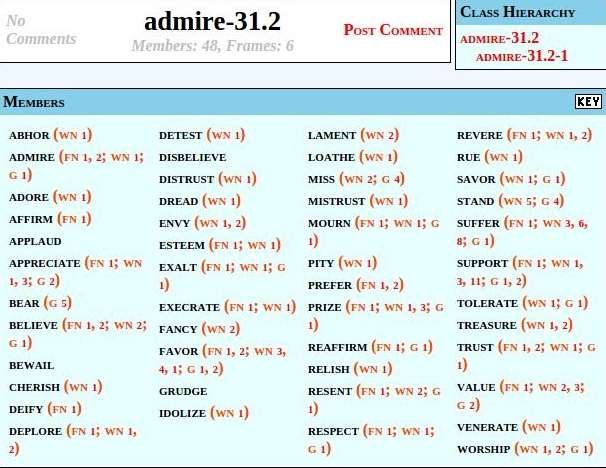
\includegraphics[width=\linewidth]{gfx/admire_class.jpg}
\caption{VerbNet's \textit{admire} class}\label{fig:admire_class}
\end{figure}

We also adapt many of the 253 members of VerbNet's \textit{amuse} class, in which the subject takes the semantic role of the cause, such as \textit{abash}, \textit{agonize}, \textit{appall}, etc. as these are equally evokative of emotions.

\subsubsection{FrameNet}

FrameNet \cite{framenet} combines syntactic and semantic generalizations: Semantic frames represent the underlying meanings of the words, linking frame elements with their syntactic realizations.

In FrameNet, emotions are conceptualized in the \textsc{emotions} frame, which describes an Experiencer in a particular emotional State that was provoked by a Stimulus. The frame \textsc{emotions} is used by ten other frames. Of these, we investigate more closely the \textsc{desiring}, \textsc{emotion\_active}, \textsc{emotion\_directed}, and \textsc{Experiencer\_obj} frames.

In the \textsc{desiring} frame, the Experiencer desires that an Event occur. We derive 20 verbs from the \textsc{desiring} frame, all of whom we label with anticipation. In the \textsc{experiencer\_obj} frame, some phenomenon (the Stimulus) provokes a particular emotion in the Experiencer. Experiencer and Stimulus (cause) are core frame elements, making this frame ideal for our purposes. We derive 132 verbs from this frame. The \textsc{emotion\_active} frame is similar to \textsc{experiencer\_obj}, but in this frame the verbs are more active. We derive 9 verbs from this frame.

Finally, the \textsc{emotion\_directed} frame focuses on adjectives and nouns describing an Experiencer's emotional response to a Stimulus. We keep a few of these, convert some into verbs, and discard the rest, resulting in 12 verbs and adjectives from this frame.

Furthermore, \textsc{emotions} is inherited by the \textsc{emotions\_by\_stimulus} frame that is in turn inherited by the \textsc{annoyance}, \textsc{emotions\_by\_possibility}, i.e. fear, \textsc{emotions\_of\_mental\_activity}, \textsc{emotions\_of\_success\_or\_failure}, \textsc{just\_found\_out}, i.e. surprise, and \textsc{others\_situation\_as\_stimulus} frames.
While these frames all refer to emotions, we have obtained most of their lexical entries already from other sources and thus don't make use of them.

\subsubsection{WordNet}

WordNet \cite{wordnet} synsets by themselves don't contain any information about sentiment or emotion. As was previously mentioned, WordNet-Affect \cite{wordnet-affect}, an additional hierarchy of affective domain labels, annotates WordNet synsets representing affective concepts in the semi-automatically augmented WordNet Domains further with affective labels.

WordNet-Affect-1.1 only contains synsets that were tagged with the label \textsc{emo(tion)} in the previous version and thus should serve our purposes. It further labels these synsets with a set of 279 distinct emotion categories, among them 'exotic' emotions such as \textit{defeatism}, \textit{self-depreciation}, \textit{puppy-love}, etc. These categories are hierarchically connected via \texttt{is-a} relations, which we map to Plutchik's eight emotions.

Given the ID listed in the WordNet-Affect-1.1 synsets, we retrieve the respective WordNet-3.0 synset lemmas using NLTK toolkit \cite{nltk} and the corresponding category. As WordNet focuses on nouns, adjectives, verbs, and adverbs are all listed with the noun that they are derived from. For these, we thus retrieve the category of the corresponding noun. This way, we produce 784 noun-, adjective-, verb-, and adverb synsets labelled with Plutchik's eight emotions. We investigate these and make use of the verb and adjective synonyms that indicate the emotion holder as well as the cause.

SentiWordNet \cite{sentiwordnet}, conversely, does not prove as helpful, as we require a finer granularity than the positivity, negativity, and subjectivity scores it assigns to WordNet synsets.

\subsection{Summary}

We give an overview of the number of patterns we extracted from each source in \ref{tab:patterns-from-sources}.

\begin{table}[]
\centering
\begin{tabular}{l|r}
{\bf Source}                 & {\bf \# of patterns} \\\hline
Oxford English Dictionary    & 24                   \\
Merriam-Webster's Dictionary & 51                   \\
Roget's Thesaurus            & 101                  \\
\citeauthor{emotion_verbs}   & 24                   \\
\citeauthor{adjective_supersenses} & 126                  \\
VerbNet                      & 178                  \\
FrameNet                     & 173                  \\
WordNet-Affect               & 123                 
\end{tabular}
\caption{Overview of the productivity of sources for pattern design}
\label{tab:patterns-from-sources}
\end{table}

We remove duplicates and manually label them with an emotion, if they were not supplied with an emotion in the resource. By adding flags to indicate if the pattern refers to a nominal phrase or a clause and if the order of subject-\textsc{experiencer}, object-\textsc{cause} is reversed, we bring them in the pattern template form depicted in \ref{ex:pattern_templates} in section \ref{sec:patterns}.

\section{Regular expression compilation} \label{sec:regex}

For the extraction, in order to match the patterns against our corpus, which we describe in section \ref{sec:corpus_selection}, we convert the pattern templates given in section \ref{sec:patterns} in regular expression patterns. We allow adjectives to be modified, but exclude negation. We add a regular expression to capture the index of a word to enable unambiguous retrieval. If the regular order specified by the second flag is reversed, e.g. for \textit{annoy}, we generate additional regular expressions that capture the passive form. These are constructed with the prepositions \textit{that} and \textit{by} and take a clause and a nominal phrase as complement respectively. Following this approach, we generate three regular expression patterns for \textit{scare} and one for \textit{be happy about}, which can be viewed in figure \ref{fig:patterns}.

\begin{figure}
\begin{lstlisting}
fear	(?! not)(?! never)scare/VB[DGPZ]/[0-9]+	NP
fear	(?<= )be/VB[PDGZ]/([0-9]+)(?! not)(?! never)( [a-z]+/RB/[0-9]+)? scare/VBN/[0-9]+ that/IN/[0-9]+	S
fear	(?<= )be/VB[PDGZ]/([0-9]+)(?! not)(?! never)( [a-z]+/RB/[0-9]+)? scare/VBN/[0-9]+ by/IN/[0-9]+	NP
joy	(?! not)(?! never)be/VB[DGPZ]/[0-9]+(?! not)(?! never)( [a-z]+/RB/[0-9]+)? happy/JJ/[0-9]+ that/IN/[0-9]+	S
\end{lstlisting}
\caption{Regex patterns for \textit{fear} and \textit{be happy about}}\label{fig:patterns}
\end{figure}

Generating regular expressions for both the active and passive form of patterns, if applicable, we arrive at 662 regular expression patterns for Plutchik's eight emotions. We match these patterns against the lemmatized, indexed, and part-of-speech tagged sentences of our corpus.

We perform a pre-filtering of these regular expressions by running an initial matching against a random sample of 2,000,000 sentences of the corpus. As we want to guarantee accuracy as well as recall, we retain patterns with an NP cause that appear at least ten times -- as these are prevalent; we retain patterns with an S cause that appear at least once.

This leaves us with 190 regular expressions, which include both active and passive forms, and 180 patterns. 

\section{Measuring annotation agreement} \label{sec:agreement}

We want to filter these 180 frequent patterns to keep only those that clearly refer to one emotion. To this end, we create an annotation task containing the 180 patterns that we hand off to three annotators (the author included). The guidelines state that each pattern should be annotated with one of Plutchik's eight emotions. We allow the annotators to label patterns with \texttt{none} in case a pattern doesn't indicate an emotion. We instruct them to label the patterns with a second choice if they think that more than one emotion applies. All three annotators are instructed to label the pattern with the degree of the assigned emotion to allow for an even finer measure of agreement. Two sample entries in the annotation task can be seen in example \ref{ex:annotation_task}, while the completed entries can be viewed in example \ref{ex:annotation_task_completed}.

\begin{align}
\begin{split}\label{ex:annotation_task}
&\textnormal{annoy}\\
&\textnormal{mourn}
\end{split}
\end{align}

\begin{align}
\begin{split}\label{ex:annotation_task_completed}
&\textnormal{annoy	anger\_III}\\
&\textnormal{mourn	sadness\_I}
\end{split}
\end{align}

We use Fleiss' kappa ($\kappa$) as a measure of inter-annotator agreement instead of the popular Cohen's $\kappa$, as Cohen's $\kappa$ only measures agreement between two annotators. Our annotators have a Fleiss' $\kappa$ of 0.65, which signifies substantial agreement according to \citeauthor{kappa}. This score is particularly significant given that $\kappa$ usually declines as the number of categories increases. The different levels of agreement can be observed in table \ref{tab:kappa_interpretation}.

\begin{table}[h]
\centering
\begin{tabular}{l|l}
Fleiss' $\kappa$ & Interpretation\\\hline
0              & poor agreement           \\
0.00 - 0.20    & slight agreement         \\
0.21 - 0.40    & fair agreement           \\
0.41 - 0.60    & moderate agreement       \\
0.61 - 0.80    & substantial agreement    \\
0.81 - 1.00    & almost perfect agreement
\end{tabular}
\caption{Fleiss' $\kappa$ values and their interpretations \cite{kappa}}
\label{tab:kappa_interpretation}
\end{table}

As can be seen in table \ref{tab:annotation}, a substantial amount, 106 of 180 expressions have been labeled unanimously with the same emotion by all three annotators. Including the second choice only increases the number slightly. 

\begin{table}
\centering
\begin{tabular}{l|r}
Annotated expressions & Number\\\hline
Unanimous emotions & 106\\
Unanimous emotions (including 2nd choice) & 119\\
Majority emotions & 163\\
Unanimous emotions + degree & 39\\
Majority emotions + degree & 131\\\hline
\textit{Total} & 180\\\hline
Fleiss' $\kappa$ & 0.65
\end{tabular}
\caption{Number of annotated expressions for different forms of agreement}
\label{tab:annotation}
\end{table}

Quite significantly, 39 expressions have been labeled with the same emotion as well as the same degree of emotion, which is a number much higher than chance\footnote{For chance, only $(\dfrac{1}{25})^{2} \cdot 180 = 0.3$ of 180 expressions would be labeled with the same degree of emotion by all annotators.} for what is essentially a 25-category classification problem (8 emotions $\cdot$ 3 degrees + 1 \texttt{none}).

\section{Final patterns} \label{sec:final_patterns}

We finally select all patterns for which we observe a majority emotion agreement, i.e. at least two of three annotators assign the same emotion. These are 163 patterns. Their distributions across all emotions can be viewed in table \ref{tab:pattern_emotion_distribution}.

\begin{table}[h]
\centering
\begin{tabular}{l|l}
{\bf Emotion} & {\bf \# of majority patterns} \\\hline
Joy           & 31\\
Trust         & 8\\
Fear          & 22\\
Surprise      & 16\\
Sadness       & 18\\
Disgust       & 14\\
Anger         & 29\\
Anticipation  & 25\\\hline
\textit{Total} & 163
\end{tabular}
\caption{Number of patterns that have been labeled by the majority with the same emotion}
\label{tab:pattern_emotion_distribution}
\end{table}

All of the patterns can be viewed in appendix \ref{ch:appendix} in table \ref{tab:majority_emotion_list}. Anger is relatively evenly distributed across its degrees (annoyance $<$ anger $<$ rage) according to Plutchik's emotion wheel (cf. figure \ref{fig:plutchik}); anticipation is harder to grasp, having been assigned almost exclusively to annoyance (rather than interest or vigilance) by the majority; fear appears in all its degrees, slightly less in terror; joy patterns are mostly labeled as joy, with a few having been attributed to ecstasy and only one to serenity; disgust, sadness, surprise, and trust never appear in their weakest form, boredom, pensiveness, distraction, and acceptance respectively.

In general, the middle tier representing the general emotion class is prevalent among the patterns labelled by the majority, with a lot of emotions not appearing in their weakest degree due to selection bias as we tended to collect patterns that were clearly indicative of one emotion.

\section{Extraction} \label{sec:extraction}

We extract the emotion holder and the cause using dependencies, which are well documented \footnote{http://nlp.stanford.edu/software/dependencies\_manual.pdf} and clearly represent the subjects, objects, and complements, which we then map to their corresponding semantic role of emotion holder or cause.\footnote{Initial experiments with extractions based on depth-first search in constituency trees exposed problems with noise and adaptation to sentential idiosyncrasies.}

We choose the Stanford collapsed dependencies for our extraction -- in lieu of regular Stanford dependencies --, as these collapse dependencies like conjunctions or prepositional objects and thus make the extraction more straight-forward, e.g. a basic dependency like \textit{prep}(cat, in) in example \ref{ex:prep_dependencies} is collapsed to \textit{prep}(cat, hat).

\begin{align}
\begin{split}\label{ex:prep_dependencies}
&\textnormal{I saw a cat in a hat. \textit{prep}(cat, in)}\\
&\textnormal{I saw a cat in a hat. \textit{prep\_in}(cat, hat)}
\end{split}
\end{align}

We extract the subject via the \texttt{nsubj} (nominal subject) or \texttt{nsubjpass} (passive nominal subject) relations and the direct object via the \texttt{dobj} relation. These relations can also be embedded in disjunctions or conjunctions, which we retrieve via the collapsed \texttt{conj\_and}, \texttt{conj\_or}, and \texttt{conj\_but} dependencies\footnote{The uncollapsed \texttt{cc} relation would increase the search depth by another relation.}. If the complement of the verb is a clause, we extract the S cause via the \texttt{ccomp} or \texttt{xcomp} relations, which are clausal complements with and without their own subjects respectively. If the verb or the adjective appears with a preposition, e.g. \textit{take pleasure in}, \textit{be proud of}, we retrieve the complement via the \texttt{pcomp} (prepositional complement) or the \texttt{pobj} (prepositional object) relation respectively. If the verb modifies the subject, e.g. \textit{a ruler loved by the people}, we extract the subject via the \texttt{partmod} relation.\footnote{As of the Stanford dependencies version 3.5.2, \texttt{partmod} has been generalized as a case of \texttt{vmod} (reduced non-finite verbal modifier)}.

Besides the emotion holder and cause, we want to extract all relevant information that might be useful for further analysis. \citeauthor{adjective_noun_pairs} clearly show that adjectives have significant emotive value by pairing positive or negative adjectives with neutral nouns to construct their adjective-noun pairs as described in \ref{sec:compositionality}. Thus we capture all modifiers as well as prepositional objects using the following relations:
\begin{aenumerate}
	\item the modifiers of the noun:
	\begin{aenumerate}
		\item \texttt{nn} (noun compound modifier), e.g. \texttt{nn}(University-10, Harvard-9)
		\item \texttt{amod} (adjectival modifier)
		\item \texttt{num} (numeric modifier)\footnote{\texttt{num} is converted to \texttt{nummod} as of version 3.5.2.}
	\end{aenumerate}
	\item the prepositional objects pertaining to the noun and the verb; collapsed prepositional objects consist of the preposition name prefixed with \texttt{prep\_}, e.g. \texttt{prep\_on}
\end{aenumerate}

We insert adjectival and numeric modifiers before the noun; we append prepositional objects prefixed by the preposition and separated by an underscore, if it is a noun, e.g. \textsc{for}:millionth\_fan. We include prepositional objects modifying the predicate of a clause in a separate bag-of-words.

Often, the emotion holder and the cause of an emotion are expressed by pronouns, which by themselves only provide limited information and generalizability. For this reason, we leverage the Stanford coreference resolution annotations of the Annotated Gigaword replacing every mention with its most representative coreferent.

To further make our results more generalizable, we tag every named entity with its named entity tag, i.e. \textsc{location}, \textsc{person}, and \textsc{organization}, replacing numbers with the \textsc{number} tag.

Dependent on the argument order, we assign the subject and the object/clause to the \textsc{experiencer} or \textsc{cause} respectively; we discard extractions where the cause still contains a pronoun, as we require our extractions to be as generalizable as possible.

Finally, we retrieve all leaves of the phrase-structure tree of the sentence that are dominated by the node of the cause (including subordinate clauses) as well as the node of the cause itself and list them in a bag-of-words tagged with their parts-of-speech. These include adjuncts and embedded relative clauses. The cause and the bag-of-words representation of the cause for the following sentence are depicted in example \ref{fig:cause-bag-of-words}:

\textit{World Health Organization experts fear the H5N1 strain will trigger a global influenza pandemic that could kill millions around the world.} (\texttt{APW\_ENG\_20050303.0369/8}).

\begin{figure}
\begin{lstlisting}
h5n1 strain	trigger global influenza pandemic
[the/DT, h5n1/JJ, strain/NN, will/MD, trigger/VB, a/DT, global/JJ, influenza/NN, pandemic/NN, that/WDT, could/MD, kill/VB, million/NNS, around/IN, the/DT, world/NN]
\end{lstlisting}
\caption{Extracted cause and bag-of-words of the cause from an example sentence}\label{fig:cause-bag-of-words}
\end{figure}

While the cause focuses on the main arguments of the complement, the bag-of-words includes the subordinate clause \textit{that could kill millions around the world}, which provides additional information for the source of the emotion.

\section{Representation of extractions} \label{sec:representation}

Using this pattern-based extraction approach, we obtain from the following sentences the extractions listed in figure \ref{fig:extractions} respectively (with tabs as delimiters):

\begin{itemize}[noitemsep,nolistsep]
	\item \textit{The countries had engaged in a multimillion-dollar battle to host the tournament, with Japan relying on its economic clout and South Korea relying on its superior soccer pedigree.}
	\item \textit{The Japanese, who expected to win the right to host the tournament, were dismayed}.
\end{itemize}

\begin{figure}
\begin{lstlisting}
NYT_ENG_19960601.0010/1	trust	rely on	Japan/LOCATION	economic clout					[its/PRP$, economic/JJ, clout/NN]
NYT_ENG_19960601.0010/9	anticipation	expect	Japanese				win	right		[to/TO, win/VB, the/DT, right/NN, to/TO, host/VB, the/DT, tournament/NN]
\end{lstlisting}
\caption{Extractions with NP and S cause}\label{fig:extractions}
\end{figure}

In both examples, Japan is the emotion holder. In the first instance, the cause is a nominal phrase extracted via the \texttt{dobj} relation, while in the second one, the cause is a clause extracted using the \texttt{xcomp} relation. We provide the following properties in ascending order of column index:

\begin{aenumerate}
	\item a unique identifier for each extraction created by concatenating the Annotated Gigaword document ID with the index of the sentence in that document;
	\item the emotion;
	\item the pattern that produced the extraction;
	\item the emotion holder;
	\item the NP cause of the emotion (can be empty);
	\item the subject of the S cause of the emotion (can be empty);
	\item the predicate of the S cause of the emotion (can be empty);
	\item the direct object of the S cause of emotion (can be empty);
	\item prepositional objects modifying the predicate of the S cause (can be empty); and
	\item a bag-of-words representation of the cause, tagged with parts-of-speech.
\end{aenumerate}

As we also collect the full propositions, we can easily cross-reference extractions via the ID to extract collocations. 